\section{Ejercicio 8}

\subsection{Enunciado}
Resuelva:

\begin{enumerate}[a)]
\item Realice tareas de prueba para comparar los schedulers \textbf{Round Robin}, \textbf{FIFO}, \textbf{SJF}, \textbf{RSJF}.

\item Compárelas según la \textbf{latencia}, \textbf{waiting time}, \textbf{turnaround}.
\newline
Realice gráficos y tablas comparativas para exponer los resultados obtenidos.

\item Escriba una breve conclusión.

\end{enumerate}


\subsection{Resolución}

Para este ejercicio se pedía realizar tareas de prueba para comparar los scheduleres \emph{Round Robin}, \emph{FCFS}, \emph{SJF} y \emph{RSJF}.

Luego, realizar comparaciones según latencia, waiting time y turnaround, realizar gráficos y tablas para exponer los resultados y dar una conclusión.

Como los schedulers \emph{SJF} y \emph{RSJF} sólo toman tareas del tipo TaskCPU, los lotes generados para los experimentos son con este tipo de tareas.

También, en los experimentos el costo de cambiar de contexto es de dos y el costo de cambiar un proceso de núcleo es de uno.

\subsection{Primera Prueba}

Para esta prueba utilizamos el lote de tareas \textbf{ej8lote1}, en donde estas son lanzadas en al mismo tiempo al comienzo de la ejecución. Los tiempos tomados para ellas son 5, 7, 3, 11 y 2.

La cantidad de cores utilizados en este caso es de uno. Y, en el caso de \emph{Round Robin} y \emph{RSJF}, el quantum dado es 3.

Lo que intentamos ver en esta prueba es, dado este lote de tareas, el comportamiento, velocidad en ejecutar y terminar estas con los schedulers implementados.

Los gráficos obtenidos son:

\begin{figure}[!h]
	\begin{center}
		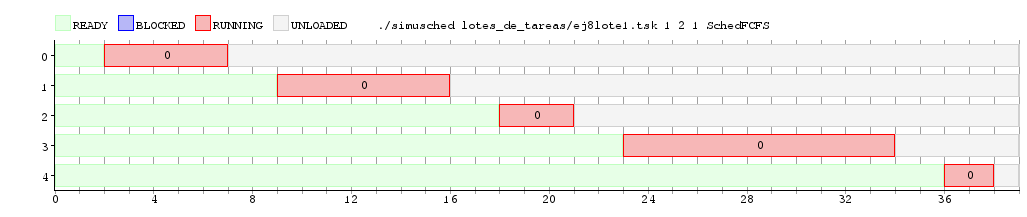
\includegraphics[width=500px]{imagenes/ej8_prueba1_fcfs.png}
		\caption{Ejecución del lote \emph{ej8lote1} con scheduler FCFS.}
		\label{fig:grafico_ej8_prueba1_fcfs}
	\end{center}
\end{figure}

\begin{figure}[!h]
	\begin{center}
		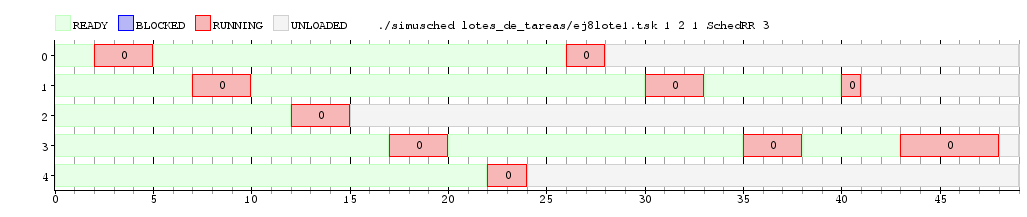
\includegraphics[width=500px]{imagenes/ej8_prueba1_rr.png}
		\caption{Ejecución del lote \emph{ej8lote1} con scheduler Round Robin.}
		\label{fig:grafico_ej8_prueba1_rr}
	\end{center}
\end{figure}

\begin{figure}[!h]
	\begin{center}
		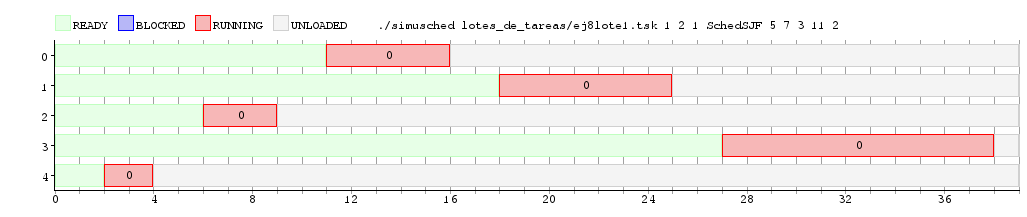
\includegraphics[width=500px]{imagenes/ej8_prueba1_sjf.png}
		\caption{Ejecución del lote \emph{ej8lote1} con scheduler SJF.}
		\label{fig:grafico_ej8_prueba1_sjf}
	\end{center}
\end{figure}

\begin{figure}[!h]
	\begin{center}
		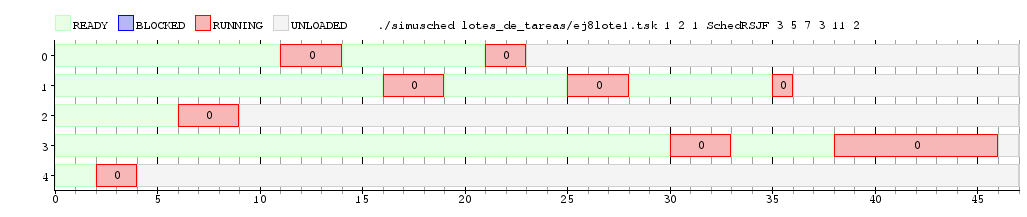
\includegraphics[width=500px]{imagenes/ej8_prueba1_rsjf.png}
		\caption{Ejecución del lote \emph{ej8lote1} con scheduler RSJF.}
		\label{fig:grafico_ej8_prueba1_rsjf}
	\end{center}
\end{figure}

%LATENCIA PROMEDIO
\begin{center}
	\begin{tabular}{|c|c|c|c|}
		\hline
		\multicolumn{4}{|c|}{\large{\textbf{Latencia Promedio}}} \\
		\hline
		\textbf{FCFS} & \textbf{Round Robin} & \textbf{SJF} & \textbf{RSJF} \\
		\hline
		17,6 & 12 & 12,8 & 13 \\
		\hline
	\end{tabular}
\end{center}

%WAITING TIME PROMEDIO
\begin{center}
	\begin{tabular}{|c|c|c|c|}
		\hline
		\multicolumn{4}{|c|}{\large{\textbf{Waiting Time Promedio}}} \\
		\hline
		\textbf{FCFS} & \textbf{Round Robin} & \textbf{SJF} & \textbf{RSJF} \\
		\hline
		17,6 & 25,6 & 12,8 & 18 \\
		\hline
	\end{tabular}
\end{center}

%TIEMPO TOTAL DE EJECUCION PROMEDIO
\begin{center}
	\begin{tabular}{|c|c|c|c|}
		\hline
		\multicolumn{4}{|c|}{\large{\textbf{Tiempo Total De Ejecución Promedio}}} \\
		\hline
		\textbf{FCFS} & \textbf{Round Robin} & \textbf{SJF} & \textbf{RSJF} \\
		\hline
		23,2 & 31,2 & 18,4 & 23,6 \\
		\hline
	\end{tabular}
\end{center}

BREVE COMENTARIO SOBRE DATOS OBTENIDOS

AHORA CON DOS CORES (QUANTUM 3 PARA CADA UNO PARA RR Y RSJF)

\begin{figure}[!h]
	\begin{center}
		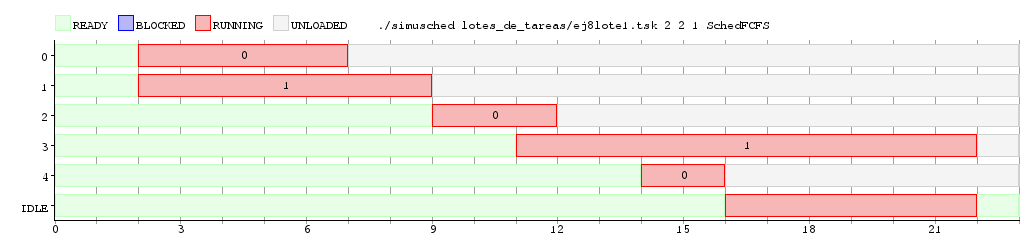
\includegraphics[width=500px]{imagenes/ej8_prueba1_fcfs2.png}
		\caption{Ejecución del lote \emph{ej8lote1} con scheduler FCFS con 2 cores.}
		\label{fig:grafico_ej8_prueba1_fcfs2}
	\end{center}
\end{figure}

\newpage

\begin{figure}[!h]
	\begin{center}
		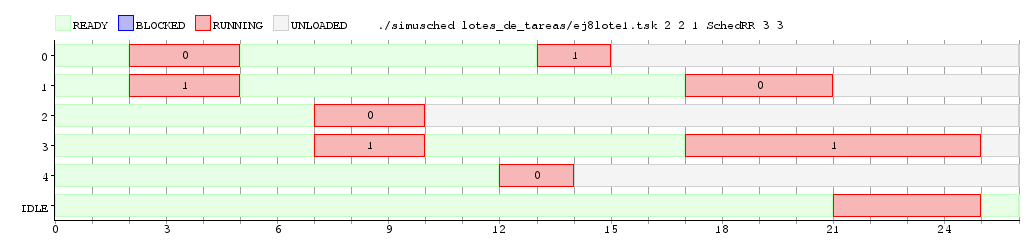
\includegraphics[width=500px]{imagenes/ej8_prueba1_rr2.png}
		\caption{Ejecución del lote \emph{ej8lote1} con scheduler Round Robin con dos cores.}
		\label{fig:grafico_ej8_prueba1_rr2}
	\end{center}
\end{figure}

\begin{figure}[!h]
	\begin{center}
		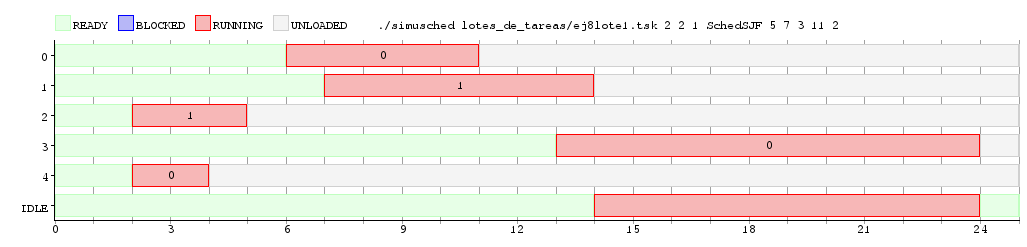
\includegraphics[width=500px]{imagenes/ej8_prueba1_sjf2.png}
		\caption{Ejecución del lote \emph{ej8lote1} con scheduler SJF con dos cores.}
		\label{fig:grafico_ej8_prueba1_sjf2}
	\end{center}
\end{figure}

\begin{figure}[!h]
	\begin{center}
		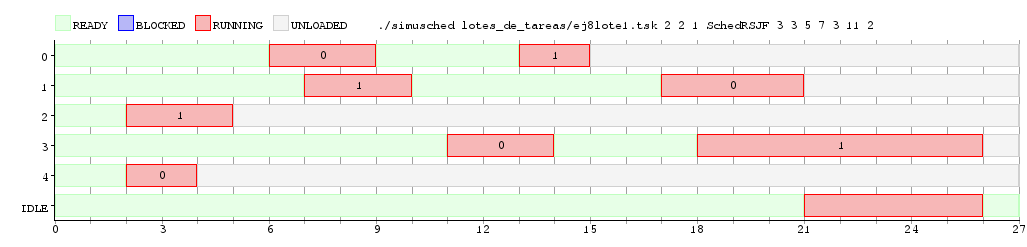
\includegraphics[width=500px]{imagenes/ej8_prueba1_rsjf2.png}
		\caption{Ejecución del lote \emph{ej8lote1} con scheduler RSJF con dos cores.}
		\label{fig:grafico_ej8_prueba1_rsjf2}
	\end{center}
\end{figure}

%LATENCIA PROMEDIO
\begin{center}
	\begin{tabular}{|c|c|c|c|}
		\hline
		\multicolumn{4}{|c|}{\large{\textbf{Latencia Promedio}}} \\
		\hline
		\textbf{FCFS} & \textbf{Round Robin} & \textbf{SJF} & \textbf{RSJF} \\
		\hline
		7,6 & 6 & 6 & 5,6 \\
		\hline
	\end{tabular}
\end{center}

%WAITING TIME PROMEDIO
\begin{center}
	\begin{tabular}{|c|c|c|c|}
		\hline
		\multicolumn{4}{|c|}{\large{\textbf{Waiting Time Promedio}}} \\
		\hline
		\textbf{FCFS} & \textbf{Round Robin} & \textbf{SJF} & \textbf{RSJF} \\
		\hline
		17,6 & 11,4 & 6 & 8,6 \\
		\hline
	\end{tabular}
\end{center}

%TIEMPO TOTAL DE EJECUCION PROMEDIO
\begin{center}
	\begin{tabular}{|c|c|c|c|}
		\hline
		\multicolumn{4}{|c|}{\large{\textbf{Tiempo Total De Ejecución Promedio}}} \\
		\hline
		\textbf{FCFS} & \textbf{Round Robin} & \textbf{SJF} & \textbf{RSJF} \\
		\hline
		17,6 & 17 & 11,6 & 14,2 \\
		\hline
	\end{tabular}
\end{center}

BREVE COMENTARIO SOBRE MEJORAS

\subsection{Segunda Prueba}

Para esta prueba utilizamos el lote de tareas \textbf{ej8lote1}, en donde estas son lanzadas con una diferencia de dos ticks desde el comienzo de la ejecución. Los tiempos tomados para ellas son los mismos que los utilizados la prueba anterior.

En esta prueba, como la anterior, comenzamos utilizando un core por scheduler y, para los schedulers \emph{Round Robin} y \emph{RSJF}, el quantum dado es 3.

La cantidad de cores utilizados en este caso es de uno. Y, en el caso de \emph{Round Robin} y \emph{RSJF}, el quantum dado es 3.

En este caso, intentamos ver el comportamiento de los schedulers en donde las tareas van apareciendo con una frecuencia constante.

Los graficos obtenidos son:

\begin{figure}[!h]
	\begin{center}
		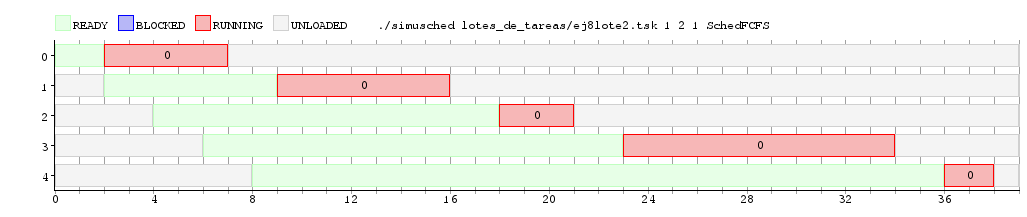
\includegraphics[width=500px]{imagenes/ej8_prueba2_fcfs.png}
		\caption{Ejecución del lote \emph{ej8lote2} con scheduler FCFS.}
		\label{fig:grafico_ej8_prueba2_fcfs}
	\end{center}
\end{figure}

\begin{figure}[!h]
	\begin{center}
		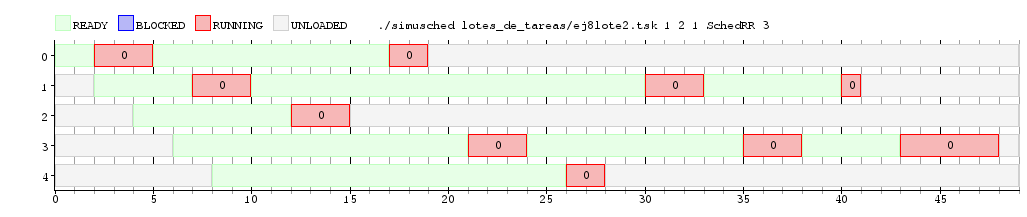
\includegraphics[width=500px]{imagenes/ej8_prueba2_rr.png}
		\caption{Ejecución del lote \emph{ej8lote2} con scheduler Round Robin.}
		\label{fig:grafico_ej8_prueba2_rr}
	\end{center}
\end{figure}

\begin{figure}[!h]
	\begin{center}
		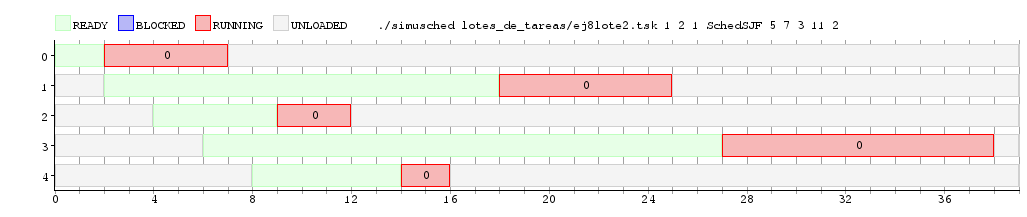
\includegraphics[width=500px]{imagenes/ej8_prueba2_sjf.png}
		\caption{Ejecución del lote \emph{ej8lote2} con scheduler SJF.}
		\label{fig:grafico_ej8_prueba2_sjf}
	\end{center}
\end{figure}

\newpage

\begin{figure}[!h]
	\begin{center}
		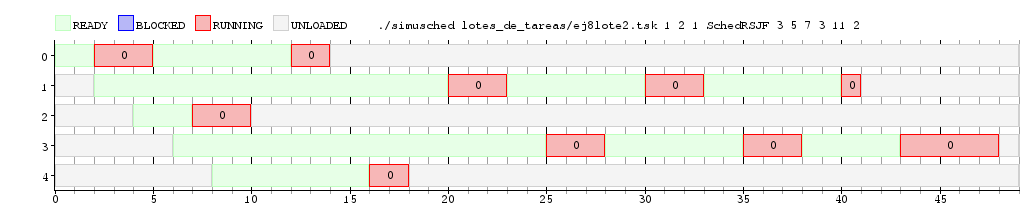
\includegraphics[width=500px]{imagenes/ej8_prueba2_rsjf.png}
		\caption{Ejecución del lote \emph{ej8lote2} con scheduler RSJF.}
		\label{fig:grafico_ej8_prueba2_rsjf}
	\end{center}
\end{figure}

%LATENCIA PROMEDIO
\begin{center}
	\begin{tabular}{|c|c|c|c|}
		\hline
		\multicolumn{4}{|c|}{\large{\textbf{Latencia Promedio}}} \\
		\hline
		\textbf{FCFS} & \textbf{Round Robin} & \textbf{SJF} & \textbf{RSJF} \\
		\hline
		11,2 & 6 & 8,8 & 8,4 \\
		\hline
	\end{tabular}
\end{center}

%WAITING TIME PROMEDIO
\begin{center}
	\begin{tabular}{|c|c|c|c|}
		\hline
		\multicolumn{4}{|c|}{\large{\textbf{Waiting Time Promedio}}} \\
		\hline
		\textbf{FCFS} & \textbf{Round Robin} & \textbf{SJF} & \textbf{RSJF} \\
		\hline
		11,2 & 20,6 & 14,8 & 13 \\
		\hline
	\end{tabular}
\end{center}

%TIEMPO TOTAL DE EJECUCION PROMEDIO
\begin{center}
	\begin{tabular}{|c|c|c|c|}
		\hline
		\multicolumn{4}{|c|}{\large{\textbf{Tiempo Total De Ejecución Promedio}}} \\
		\hline
		\textbf{FCFS} & \textbf{Round Robin} & \textbf{SJF} & \textbf{RSJF} \\
		\hline
		17,6 & 20,6 & 10 & 16,6 \\
		\hline
	\end{tabular}
\end{center}

BREVE COMENTARIO SOBRE DATOS OBTENIDOS

AHORA CON DOS CORES (QUANTUM 3 PARA CADA UNO PARA RR Y RSJF)

\begin{figure}[!h]
	\begin{center}
		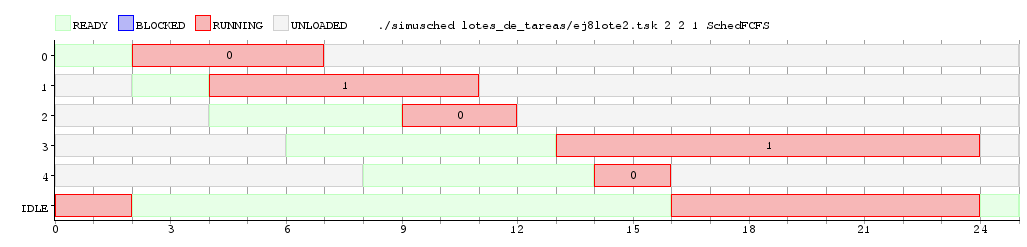
\includegraphics[width=500px]{imagenes/ej8_prueba2_fcfs2.png}
		\caption{Ejecución del lote \emph{ej8lote2} con scheduler FCFS con 2 cores.}
		\label{fig:grafico_ej8_prueba2_fcfs2}
	\end{center}
\end{figure}

\begin{figure}[!h]
	\begin{center}
		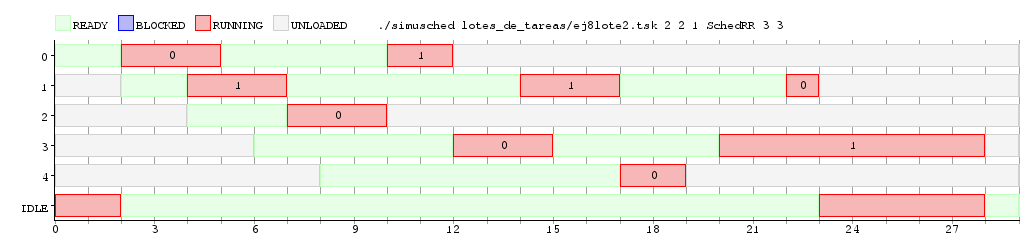
\includegraphics[width=500px]{imagenes/ej8_prueba2_rr2.png}
		\caption{Ejecución del lote \emph{ej8lote2} con scheduler Round Robin con dos cores.}
		\label{fig:grafico_ej8_prueba2_rr2}
	\end{center}
\end{figure}

\newpage

\begin{figure}[!h]
	\begin{center}
		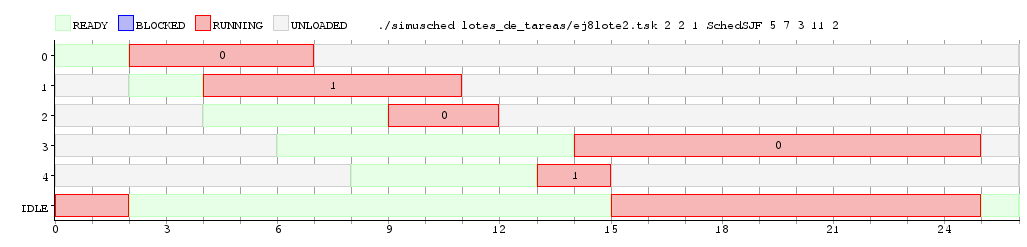
\includegraphics[width=500px]{imagenes/ej8_prueba2_sjf2.png}
		\caption{Ejecución del lote \emph{ej8lote2} con scheduler SJF con dos cores.}
		\label{fig:grafico_ej8_prueba2_sjf2}
	\end{center}
\end{figure}

\begin{figure}[!h]
	\begin{center}
		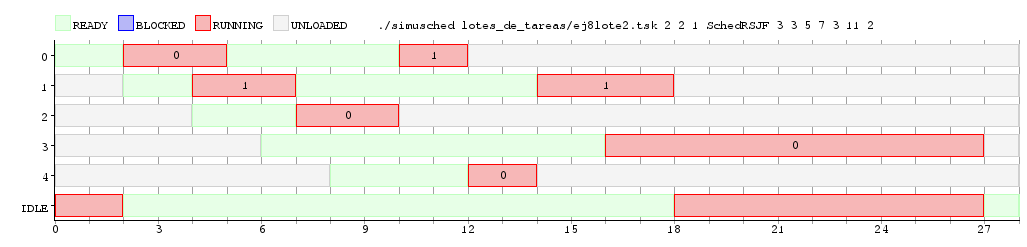
\includegraphics[width=500px]{imagenes/ej8_prueba2_rsjf2.png}
		\caption{Ejecución del lote \emph{ej8lote2} con scheduler RSJF con dos cores.}
		\label{fig:grafico_ej8_prueba2_rsjf2}
	\end{center}
\end{figure}

%LATENCIA PROMEDIO
\begin{center}
	\begin{tabular}{|c|c|c|c|}
		\hline
		\multicolumn{4}{|c|}{\large{\textbf{Latencia Promedio}}} \\
		\hline
		\textbf{FCFS} & \textbf{Round Robin} & \textbf{SJF} & \textbf{RSJF} \\
		\hline
		4,4 & 4,4 & 4,4 & 4,2 \\
		\hline
	\end{tabular}
\end{center}

%WAITING TIME PROMEDIO
\begin{center}
	\begin{tabular}{|c|c|c|c|}
		\hline
		\multicolumn{4}{|c|}{\large{\textbf{Waiting Time Promedio}}} \\
		\hline
		\textbf{FCFS} & \textbf{Round Robin} & \textbf{SJF} & \textbf{RSJF} \\
		\hline
		4,4 & 8,8 & 4,4 & 6,6 \\
		\hline
	\end{tabular}
\end{center}

%TIEMPO TOTAL DE EJECUCION PROMEDIO
\begin{center}
	\begin{tabular}{|c|c|c|c|}
		\hline
		\multicolumn{4}{|c|}{\large{\textbf{Tiempo Total De Ejecución Promedio}}} \\
		\hline
		\textbf{FCFS} & \textbf{Round Robin} & \textbf{SJF} & \textbf{RSJF} \\
		\hline
		10 & 14,4 & 10 & 12,2 \\
		\hline
	\end{tabular}
\end{center}

BREVE COMENTARIO SOBRE MEJORAS
